\documentclass
{llncs}




%\makeatletter
%\def\input@path{{../}}
%\makeatother
%
% Estos son los paquetes q ocupan todas las versiones del paper (normal y eprint)
%\usepackage{setspace}
\usepackage{amsmath,amsfonts,amssymb,amstext}
\usepackage{mathtools}
\usepackage{latexsym,ifthen}
\usepackage{bbm,url}
\usepackage{float}
\usepackage{bm}
\usepackage{xspace}
%\usepackage[usenames,dvipsnames]{color}
\usepackage{tikz}
\usepackage{xspace}
\usetikzlibrary{arrows,chains,matrix,positioning,scopes,patterns}
\usepackage{authblk}
%\usepackage[pdftex,pagebackref]{hyperref}
\usepackage{multirow}
\usepackage{wasysym}
%\usepackage{enumitem}
\usepackage[font=scriptsize]{caption}
% Temporal
\usepackage{soul}

\usepackage{enumerate}


\newif\iffull
\fullfalse
%\usepackage{fullpage}
\input{preamble}


\author{Alonso Gonz\'alez \inst{1}}
\institute{Mi casita}

\title{A Ring Signature of size $O(\sqrt[3]{n})$ without Random Oracles}
\begin{document}
%\begin{doublespace}

\maketitle
%\vspace*{-.5cm}
\begin{abstract}
    % !TEX root = ./main-ring-signature.tex

Ring signatures, introduced by Rivest, Shamir and Tauman (ASIACRYPT 2001), allow to sign a message on behalf of a set of users while guaranteeing authenticity and anonymity. In terms of efficiency, two of the shortest ring signatures are of size $\Theta(\log n)$, where $n$ is the number of users, and are due to Groth and Kohlweiss (EUROCRYPT 2015) and Libert et al.~(EUROCRYPT 2016). An even shorter ring signature, of size independent from the number of users, was recently proposed by Malavolta and  Schr\"oder (ASIACRYPT 2017).
The former schemes are both proven secure in the random oracle model while the later requires non-falsifiable assumptions.
Under more standard assumptions Chase and Lysyanskaya proposed a constant-size, but impractical, size ring signature that requires simulation sound NIZK proofs systems for circuit satisfiability.
The most practical construction remains the one of Chandran et al.~(ICALP 2007) with a signature of size $\Theta(\sqrt{n})$ and security based on the Diffie-Hellman assumption in bilinear groups.

In this work we construct an asymptotically shorter ring signature without random oracles or non-falsifiable assumptions. Its security is proven under the hardness of the permutation pairing assumption, a falsifiable assumption in bilinear groups introduced by Groth and Lu (ASIACRYPT 2007).
 Each signature comprises $\Theta(\sqrt[3]{n})$ group elements, signing a message requires computing $\Theta(\sqrt[3]{n})$ exponentiations, and verifying a signature requires $\Theta(n^{2/3})$ pairing operations. To the best of our knowledge, this is the first practical ring signature with $o(\sqrt{n})$ signatures and sublinear verification time.

\end{abstract} 

\section{Introduction}
    % !TEX root = ../main-ring-signature.tex

Ring signatures, introduced by Rivest, Shamir and Tauman, \cite{AC:RivShaTau01}, allow to anonymously sign a message on behalf of a ring of users $R=\{P_1,\ldots,P_n\}$, only if the signer belongs to that ring. That is, no one outside $R$ can forge a valid signature and  an honestly computed signature reveals (essentially) no information about the actual signer.  
Unlike other similar primitives such as group signatures \cite{EC:ChaVan91}, ring signatures are not coordinated: each user generates secret/public keys on his own --- i.e.~no central authorities --- and might sign on behalf of a ring without the approval or assistance of the other members.

The original motivation for ring signatures was anonymous leakage of secrets. Suppose a high rank officer wants to leak some sensitive document to a journalist without revealing its identity. To do so, it signs this document using a ring signature where the ring contains all other high rank officers. The journalist is convinced that some high rank officer signed the document, but it has no clue who.

Besides this hypothetical application, with the advent of cryptocurrencies, ring signatures have found new and more practical applications. For example, for spending a coin in Monero, a user form a ring from public keys in the blockchain to issue a ring signature on the transaction. Thereby, the anonymity properties of the ring signature guarantee untraceability and fungibility. 
Given the practical usefulness of ring signatures, it becomes crucial to study and improve its efficiency.

\subsection{Related Work}
The efficiency of a ring signature might be splitted in three parameters: the signature size, the cost (time) of computing a signature, and the cost (time) of verifying a signature. Among these metrics, the signature size has received the most attention and improvements in the size usually imply improvement on the other metrics.
In terms of ring size, one the most efficient constructions have signature size logarithmic in the size of the ring \cite{EC:GroKoh15,EC:LLNW16}. However,  both constructions rely on the {random oracle model}, which is an idealization of hash functions with known theoretical inconsistencies \cite{FOCS:GolKal03}. Malavolta et al.~constructed a constant size ring signature without random oracles \cite{AC:MalSch17} using SNARKS \cite{EC:GGPR13,AC:DFGK14,EC:Groth16} as a subroutine. However, SNARKS are known to require controversial non-falsifiable assumptions such as the knowledge of exponent assumption  \cite{STOC:GenWic11,C:Naor03} .
In spite of their limitations, in practice random oracles or non-falsifiable assumptions might be acceptable. However, it is still interesting and challenging to explore practical constructions from more standard assumptions.

Chase and Lysyanskaya proposed a ring signature scheme whose size, although independent from the number of users, is large enough for consider it practical \cite{C:ChaLys06}.%\footnote{This works seems to has gone unnoticed in the ring signature literature. In fact, to the best of our knowledge, the only recent work citing it is \cite{AC:MalSch17}.}
After introducing
signatures of knowledge, they use this primitive to construct ring signatures from accumulators, following Dodis et al.~\cite{EC:DKNS04}. The scheme description is only sketched and no proof of security is given but, for fairness and as also noted in \cite{AC:MalSch17}, their work is previous to the (now standard) formal definition of ring signatures of Bender et al.~\cite{TCC:BenKatMor06}. Their scheme goes as follows.
Given a ring of RSA public keys $R = \{(N,y_1),...,(N,y_n)\}\subseteq \Z_{\phi(N)}$, one can compute an accumulated value $a = g^{\prod_{i=1}^n y_i}$ and a witness $w_i = a^{-y_i} \mod N$ that $y_i$ is accumulated in $a$, which can be verified checking if $a = w_i^{y_i} \mod N$. A ring signature on a message $m$ is computed as a signature on $m$ of knowledge of $x_i,y_i\in \Z_{\phi(N)}, w_i\in \Z_N$ such that: a) $x_iy_i = 1 \mod \phi(N)$ and b)  $a = w_i^{y_i} \mod N$. However, signatures of knowledge are built on top of simulation sound NIZK which in turn is built from standard NIZK, and the only NIZK proof system for a) and b) seems to be generic NIZK for circuit satisfiability. For example, using Groth-Sahai proofs the proof will require $O(|C|)$ elements of a bilinear group, where $|C|$ is the size of the circuit for computing a) $\wedge$ b). One might expect the circuit for a) and b) to have at least $\approx 10^4$ gates\footnote{For example, in \url{https://www.cs.bris.ac.uk/Research/CryptographySecurity/MPC/}, a circuit for multiplying 32x32-bit integers requires $\approx 10^4$ gates. Our estimation is quite conservative since RSA integers should be of size $\geq 1024$, and further, one might expect a circuit for a) and b) to contain at least thousands of multiplication gates.}, and thus the proof will be of size greater than $10^4$ elements of a bilinear group.

Despite Chase and Lysyanskaya's construction, without random oracles or non-falsifiable assumptions all constructions have signatures of size linear in the size of the ring, being the sole exception the $\Theta(\sqrt{n})$ ring signature of Chandran et al.~\cite{ICALP:ChaGroSah07}. They construct a simple and nice ring signature which at its core implements a \emph{set-membersip proof}, i.e.~a proof that somme commited public key belongs to the set of public keys of the ring users. Their set-mebership proof is quite strong, in the sense that the verification keys may be even chosen by the adversary. Going a step forward, we will build a more efficient but weaker set-mebership proof which is still useful for building ring sinatures.

We note that no improvements in the
signature size have been made within a decade. In fact, although two previous works claim to construct signatures of constant \cite{ACISP:BosDasRan15} or logarithmic \cite{IET:GriSusPla16} size, in Appendix \ref{sec:rs-flawed} we show that one construction fails to give a correct proof of security and the other is in fact of size $\Theta(n)$. The only (non-asymptotic) improvements we are aware of are \cite{TCC:Rafols15,AC:GonHevRaf15}.

\subsection{Our contribution}
In this work we present the first ring signature based on bilinear groups whose signature size is asymptotically smaller than Chandran et al.'s, and whose security is proven under falsifiable assumptions and without random oracles. Our ring signature consists of $\Theta(\sqrt[3]{n})$ group elements, computing a signature requires $\Theta(\sqrt[3]{n})$ exponentiations, and verifying a signature requires $\Theta(n^{2/3})$ pairings. Our ring signature is perfectly anonymous, i.e.~it completely hides the identity of the actual signer, and is computationally infeasible to forge signatures for non-members of the ring.

The security of our construction relies on a security assumption --- the {permutation pairing assumption} --- introduced by Groth and Lu \cite{AC:GroLu07} in an unrelated setting: proofs of correctness of a shuffle. While the assumption is ``non-standard'', in the sense that is not a ``DDH like'' assumption, it is a falsifiable assumption and it was proven hard in generic symmetric bilinear groups by Groth and Lu. We work on asymmetric groups (Type III groups \cite{EPRINT:GalPatSma06}) and thus we give a natural variant of the permutation pairing assumption which we prove secure in generic asymmetric bilinear groups.

Our ring signature outperforms Chandran et al.'s in terms signature size for any $n > 144$, in terms of signature generation time for any $n>96$, and in terms of verifier efficiency for any $n>111$. However, this analysis should be taken with care, since Chandran et al.'s signature is proven secure under the decisional linear (DLin) assumption while ours is proven secure under the permutation pairing assumption. Being the permutation pairing assumption much less studied than DLin, it could be the case that our scheme would be as secure as Chandran et al.'s at higher values of the security parameter. In Table \ref{table:eff} we provide a comparison between our scheme and Chandran et al.'s.
 
\begin{table}[h]
\begin{center}
\begin{minipage}{\textwidth}
\begin{center}
%\begin{scriptsize}
\begin{tabular}{|l|l|l|}
\hline
                                           & Chandran et al.~\cite{ICALP:ChaGroSah07} & This work \\
\hline\hline
\rule{0pt}{2.5ex}CRS size                  & $9$                                       & $9$       \\ 
\rule{0pt}{2.5ex}Verification key size     & $1$                                       & $5$       \\
\rule{0pt}{2.5ex}Signature size            & $24 \sqrt{n} + 24$                        & $39 \sqrt[3]{n} + 30 \sqrt[6]{n} + 81$\\    
\rule{0pt}{2.5ex}Signature generation time & $42 \sqrt{n} + 49$                        & $69 \sqrt[3]{n} + 42 \sqrt[6]{n} + 142$\\
\rule{0pt}{2.5ex}Verification time         & $3 n + 120 \sqrt{n} + 121$                & $6 n^{2/3} + 210 \sqrt[3]{n} + 186 \sqrt[6]{n} + 411$\\
\hline 
\end{tabular}
%\end{scriptsize}
\end{center}
\caption{Comparison of Chandran et al.'s ring signature and ours for a ring of size $n$. 'Signature generation time' is measured in number of exponentiations, 'Verification time' is measured in number of pairings, and all other rows are measured in number of group elements.\label{table:eff}}
\end{minipage}
\end{center}
\end{table}


We require members of the ring to erase the random coins after generating the public/secret key pair. The reason is that the public keys contain group elements whose discrete logs are of the form $(a,a^2)$. Although this helps to embed an instance of the permutation pairing assumption in the set of (honest) public keys. It prevents oblivious sampling of the verification keys and thus, users must generate information that, when the user is corrupted, renders easy the permutation pairing assumption. We remark that this only affects unforgeability and honestly generated signatures still don't reveal any information about the signer.

Further, without erasures, it is unlikely that such adversary exists. We uphold this on the fact that our scheme is secure, without erasures, under a stronger assumption, the \emph{interactive} permutation pairing assumption, which we prove secure in generic bilinear groups.
%
%\begin{figure}[!t]
%	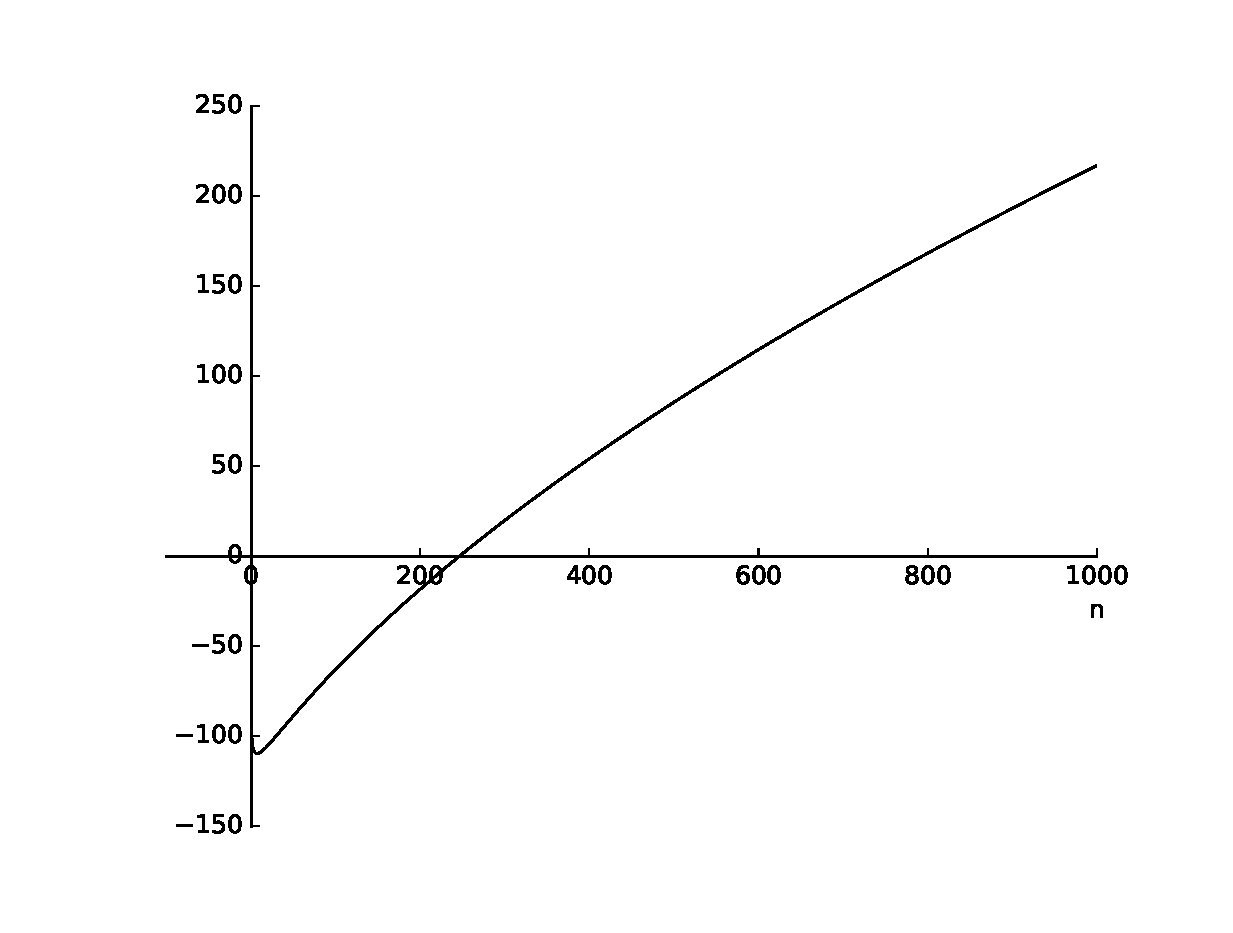
\includegraphics[scale=.25]{intro/sign_size}
%	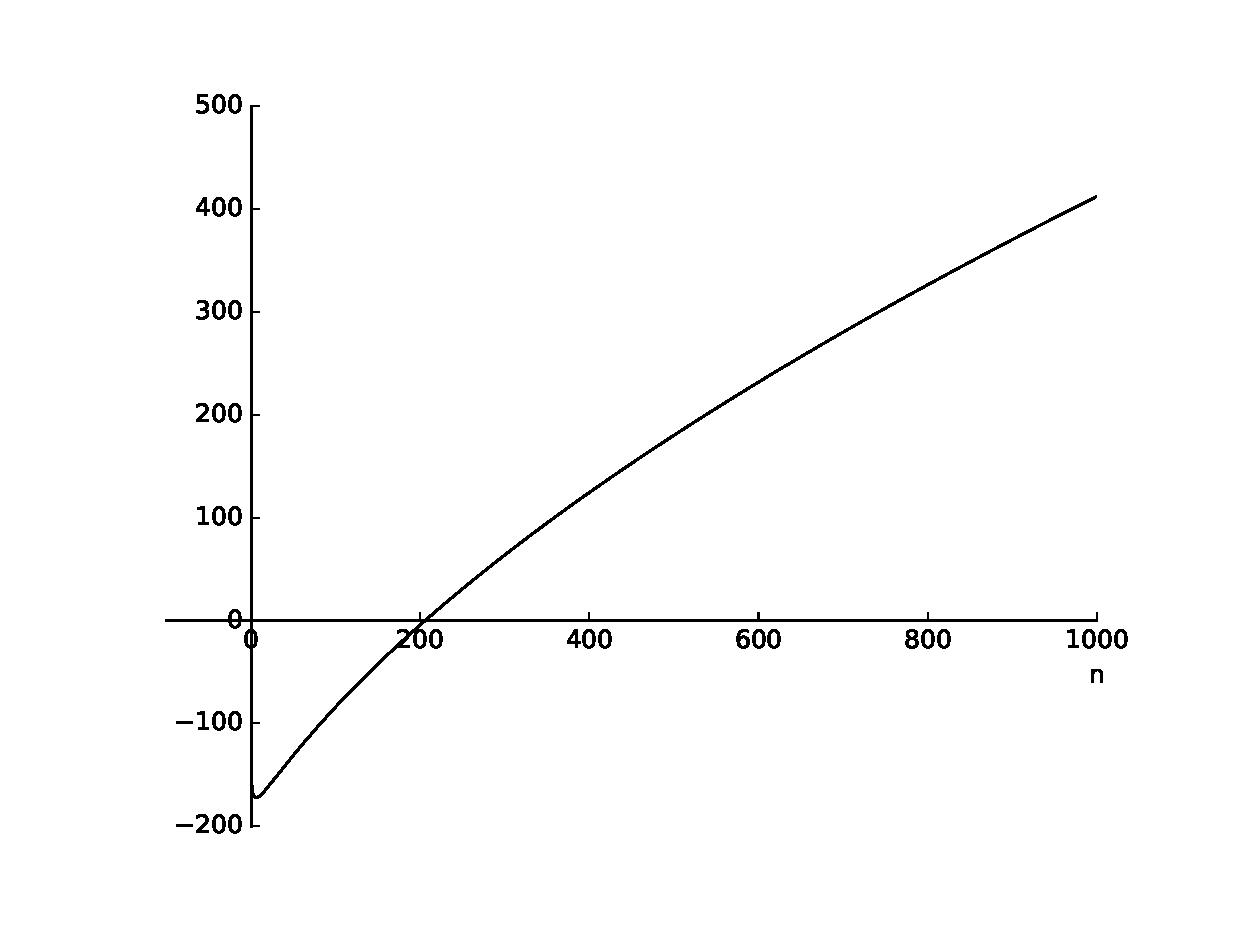
\includegraphics[scale=.25]{intro/sign_time}
%	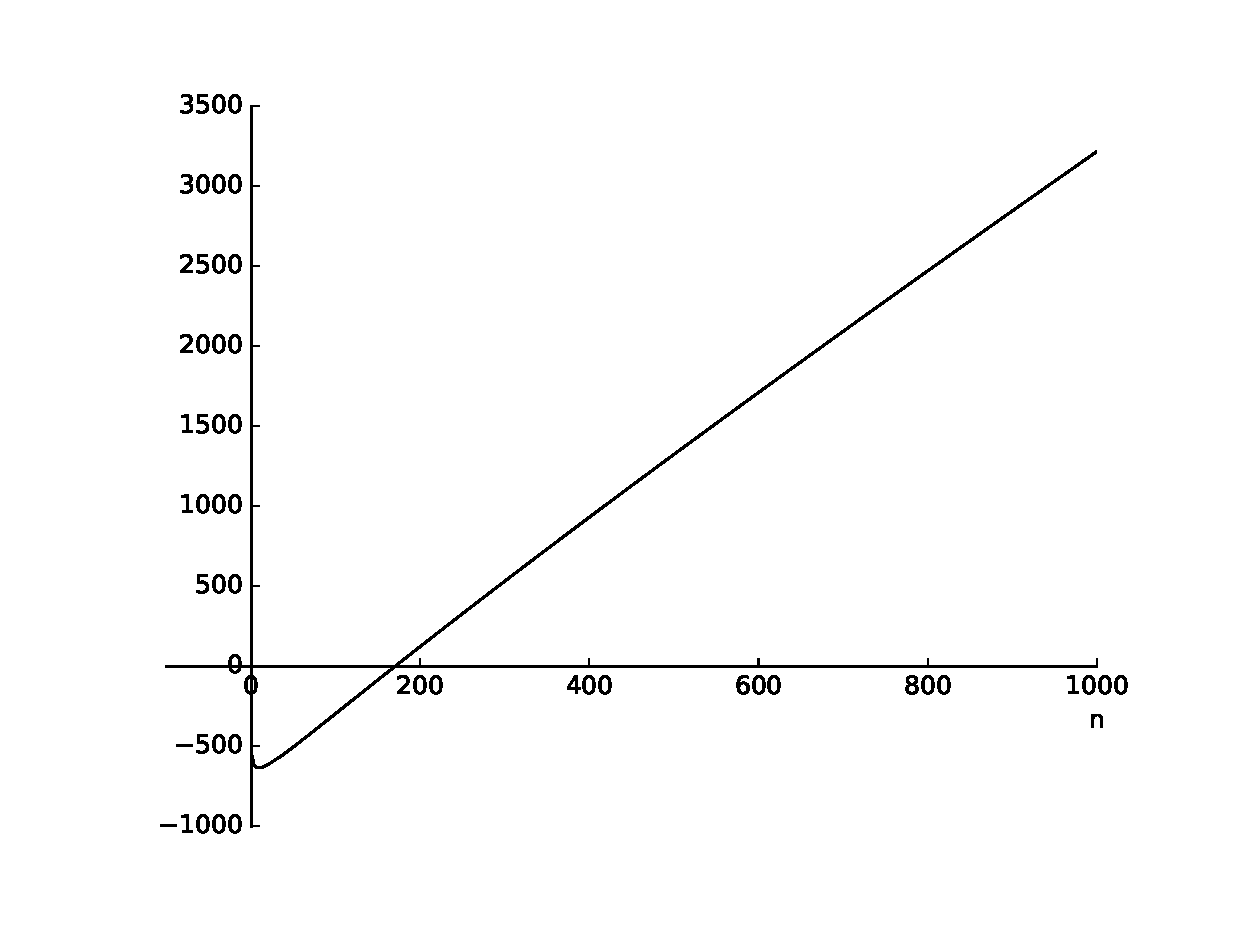
\includegraphics[scale=.25]{intro/ver_time}
%\end{figure}

    
    \subsection{Chandran et al.'s Costruction}
	
         % !TEX root = ../main-ring-signature.tex


Consider a {Boneh-Boyen signature scheme} with secret/verification keys of the form $(sk,[vk]_2)$ and a {one-time signature scheme}. The signature of the message $m$ for a ring $R=\{[vk_1]_2,\ldots,[vk_n]_2\}$ is computed as follows:
\begin{itemize}
	\item[a)] Pick a one-time signature key $(sk_\mathsf{ot},vk_\mathsf{ot})$, sign $m$ with $sk_\mathsf{ot}$, and sign $vk_\mathsf{ot}$ with $sk$.
	\item[b)] Show possession of valid signature of $vk_\mathsf{ot}$ under $[vk]_2$ using Groth-Sahai proofs.
	\item[c)] Show that $[vk]_2\in R$.
\end{itemize}
The most expensive part is c) and the core of Chandran et al.'s construction is a proof of size $\Theta(\sqrt{n})$ of c). We call this kind of proof a set-membership proof and we describe Chandran et al.'s below.
 
The proof arranges the set of verification keys on a matrix of size $m\times m$, where $m:=\sqrt{n}$, as depicted below
$$
[\matr{V}]_2:=
\begin{pmatrix}
[vk_{1,1}]_2 & \cdots & [vk_{1,m}]_2\\
\vdots     & \ddots & \vdots \\
[vk_{m,1}]_2  & \cdots & [vk_{m,m}]_2,
\end{pmatrix}
$$
where $vk_{i,j}:=vk_{(i-1)m+j}$ for $1\leq i,j \leq m$.

Let $[vk_\alpha]_2$ the verification key for which the prover wants to show that $[vk_\alpha]_2\in R$ and let $i_\alpha,j_\alpha$ such that $vk_\alpha = vk_{i_\alpha,j_\alpha}$. The prover selects the $j_\alpha$ th column of $[\matr{V}]_2$ and then the $i_\alpha$ th element of that column. To do so, the prover commits to 
\begin{enumerate}
\item $b_1,\ldots,b_m\in\bits$ such that $b_j=1$ iff $j=j_\alpha$,
\item $b'_1,\ldots,b'_m\in\bits$ such that $b'_i=1$ iff $i=i_\alpha$,
\item $[\kappa_1]_2:=[vk_{1,j_\alpha}]_2,\ldots,[\kappa_m]_2:=[vk_{m,j_\alpha}]_2$.
\end{enumerate}

Using Groth-Sahai proofs, the prover proves that
\begin{enumerate}[i.]
\item $b_1(b_1-1)=0,\ldots,b_m(b_m-1)=0,b'_1(b'_m-1)=0,\ldots,b'_m(b'_m-1)=0$,\label{eq1}
\item $\sum_{i=1}^m b_i =1$ and $\sum_{i=1}^m b'_i=1$,\label{eq2}
\item $[\kappa_1]_2=\sum_{j=1}^m b_j [vk_{1,j}]_2,\ldots,[\kappa_m]_2=\sum_{j=1}^m b_j[vk_{m,j}]_2$,\label{eq3}
\item $[vk_\alpha]_2=\sum_{i=1}^m b'_i[\kappa_i]_2$.\label{eq4}
\end{enumerate}
Equations \ref{eq1} and \ref{eq2} prove that $(b_1,\ldots,b_m)$ and $(b'_1,\ldots,b'_m)$ are unitary vectors, equation \ref{eq3} proves that $([\kappa_1]_2,\ldots,[\kappa_m]_2)^\top$ is a column of $[\matr{V}]_2$, and equation \ref{eq4} proves that $[vk_\alpha]_2$ is an element of $([\kappa_1]_2,\ldots,[\kappa_m]_2)$.

In our SXDH base ring signature we need this set-membership to show that some vector $[\vecb{s}]_2$ is the re-encryption of one of the elements of the set of commitments $S = \{[\vecb{s}]_2,\ldots,[\vecb{s}]_n\}\subseteq\GG_2$. That is, there exists some $\delta\in\Z_q$ such that $[\vecb{s}]-\delta[\vecb{v}_2]_2\in S$. The proof remains the same but now
the prover computes re-randomizations
\begin{enumerate}[1.']
\setcounter{enumi}{2}
\item[3'.] $[\vecb{\kappa}_1]_2:=[\vecb{s}_{1,j_\alpha}]_2+\delta_1[\vecb{v}_2],\ldots,[\vecb{\kappa}_m]_2:=[\vecb{s}_{m,j_\alpha}]_2+\delta_m[\vecb{v}_2]_2$.
\end{enumerate}
and Groth-Sahai proofs that
\begin{enumerate}[i.']
\setcounter{enumi}{2}
\item[iii'.] $[\vecb{\kappa}_1]_2 - \sum_{j=1}^m b_j [\vecb{s}_{1,j}]_2 = \delta_1[\vecb{v}_2]_2,\ldots,[\vecb{\kappa}_m]_2-\sum_{j=1}^m b_j[\vecb{s}_{m,j}]_2 = \delta_m[\vecb{v}_2]_2$,\label{eq3}
\item[iv'.] $[\vecb{s}]_2 - \sum_{i=1}^m b'_i[\vecb{\kappa}_i]_2  = (\delta-\delta_{i_\alpha})[\vecb{v}_2]_2$.\label{eq4}
\end{enumerate} 
    
    \subsection{Our Construction}
        
        %We propose an alternative way of obtaining a $\sqrt{n}$ ring signature. We then combine both techniques, Chandran et al. and ours, and obtain a $\sqrt[3]{n}$ signature.
%
%
%Following Chandran et al.'s approach, if we want to obtain a $m:=\sqrt[3]{n}$ proof it is natural to arrange the verification keys in $m$ matrices of size $m\times m$ (a 3d array) as depcited bellow
%$$
%\begin{pmatrix}
%[vk_{1,1,1}] & \cdots & [vk_{1,1,m}]\\
%\vdots       & \ddots & \vdots      \\
%[vk_{1,m,1}] & \cdots & [vk_{1,m,m}]
%\end{pmatrix},
%\ldots,
%\begin{pmatrix}
%[vk_{m,1,1}] & \cdots & [vk_{m,1,m}]\\
%\vdots       & \ddots & \vdots      \\
%[vk_{m,m,1}] & \cdots & [vk_{m,m,m}]
%\end{pmatrix},
%$$
%where $vk_{i,j,k}:=vk_{(i-1)m^2+(j-1)m+k}$ for $i,j,k\in[m]$.
%
%The naive approach of selecting one of this matrices and then applying Chandran et al.'s approach will end up with a proof of size $n^{2/3}$. We follow the approach of Gonzalez et al.~\cite{AC:GonHevRaf15} which aggreates the $m$ matrices into a single one selecting $\vecb{a}_1,\ldots,\vecb{a}_n$ from some distribution such that the corresponding kernel problem is hard (using the terminology of Morillo et al.~\cite{AC:MorRafVil16}). That is, compute
%$$
%[\matr{V}] := \sum_{i=1}^{m} \vecb{a}_i
%\begin{pmatrix}
%[vk_{i,1,1}] & \cdots & [vk_{i,1,m}]\\
%\vdots       & \ddots & \vdots      \\
%[vk_{i,m,1}] & \cdots & [vk_{i,m,m}]
%\end{pmatrix}
%$$

In our scheme the secret/verification keys of party $P$ are $(sk,\vecb{vk})$, where $\vecb{vk}=([vk],[\vecb{a}],\vecb{a}[vk])$, $(sk,[vk])$ are secret/verification keys of the Boneh-Boyen signature scheme, and $\vecb{a}\in\Z_q^2$ is chosen independently for each key from some distribution $\mathcal{Q}$ to be specified later. Suppose that $\vecb{vk}$ is the $\alpha$ th element in the ring $R=\{\vecb{vk}_{1,1,1},\ldots,\vecb{vk}_{m,m,m}\}$, where $\vecb{vk}_{i,j,k}=\vecb{vk}_{(i-1)m^2+(j-1)m+k}$ for $i,j,k\in[m],m:=\sqrt[3]{n}$. Let $i_\alpha,j_\alpha,k_\alpha\in[m]$ such that $\vecb{vk}_\alpha = \vecb{vk}_{i_\alpha,j_\alpha,k_\alpha}$. Consider the sets
\begin{align*}
&S:=\{[\vecb{s}_1],\ldots,[\vecb{s}_{n^{2/3}}]\}:=\left\{\sum_{i\in[m]}[\vecb{a}_{i,1,1}],\ldots,\sum_{i\in[m]}[\vecb{a}_{i,m,m}]\right\}\text{ and }\\
&S':=\{[\vecb{s}'_1],\ldots,[\vecb{s}'_{n^{2/3}}]\}:=\left\{\sum_{i\in[m]}\vecb{a}_{i,1,1}[vk_{i,1,1}],\ldots,\sum_{i\in[m]}\vecb{a}_{i,m,m}[vk_{i,m,m}]\right\}.
\end{align*}

The prover commits to $[\vecb{x}]=[\vecb{s}_\mu]$ and $[\vecb{y}]=[\vecb{s}'_{\mu'}]$, for $\mu=\mu'=(j_\alpha-1)m+k_\alpha$, and shows, using (twice) the set-membership proof of Chandran et al., that $[\vecb{x}]\in S$ and that $[\vecb{y}]\in S'$, 
The prover also needs to assure that $\mu=\mu'$, which can be done reutilizing the commitment to $\mu$ (in fact to its binary representation) used in the proof that $[\vecb{x}]\in S$ in the proof that $[\vecb{y}]\in S'$. Since both sets are of size $n^{2/3}$, the two set membership proofs are of size $\Theta(\sqrt[3]{n})$.
 
Now that the prover has commited to elements $[\vecb{x}]=\sum_{i\in[m]}[\vecb{a}_{i,j_\alpha,k_\alpha}]$ and $[\vecb{y}]=\sum_{i\in[m]}\vecb{a}_{i,j_\alpha,k_\alpha}[vk_{i,j_\alpha,k_\alpha}]$, it additionally commits to $[\kappa_1]:=[vk_{1,j_\alpha,k_\alpha}],\allowbreak\ldots,\allowbreak[\kappa_m]:=[vk_{m,j_\alpha,k_\alpha}]$ and $[\vecb{z}_1]:=[\vecb{a}_{1,j_\alpha,k_\alpha}],\ldots,[\vecb{z}_m]:=[\vecb{a}_{m,j_\alpha,k_\alpha}]$. The prover now gives a proof that
\begin{equation}
\sum_{i\in[m]}[\vecb{z}_i][\kappa_i]=[\vecb{y}][1]. \label{eq:verif1}
\end{equation}

Assume for a while that $\vecb{z}_1,\ldots,\vecb{z}_m$ is a permutation of $\vecb{a}_{1,j_\alpha,k_\alpha},\ldots,\vecb{a}_{m,j_\alpha,k_\alpha}$, that is $\vecb{z}_i=\vecb{a}_{\pi(i),j_\alpha,k_\alpha}$, $i\in[m]$, for some permutation $\pi\in S_m$. Therefore, equation (\ref{eq:verif1}) implies that
\begin{align*}
\sum_{i\in[m]}[\vecb{z}_i][\kappa_i]&=\sum_{i\in[m]}[\vecb{a}_{\pi(i),j_\alpha,k_\alpha}][\kappa_i]=\sum_{i\in[m]}[\vecb{a}_{i,j_\alpha,k_\alpha}][\kappa_{\pi^{-1}(i)}]\\
&=\sum_{i\in[m]}[\vecb{a}_{i,j_\alpha,k_\alpha}][vk_{i,j_\alpha,k_\alpha}].
\end{align*}
Then $\kappa_1,\ldots,\kappa_m$ is a permutation of $vk_{1,j_\alpha,k_\alpha},\ldots,vk_{m,j_\alpha,k_\alpha}$ (the same defined by $\vecb{z}_1,\ldots,\vecb{z}_m$), unless $(\kappa_{\pi^{-1}(1)}-{vk_{1,j_\alpha,k_\alpha}),\ldots,\kappa_{\pi^{-1}(m)}-vk_{m,j_\alpha,k_\alpha})})^\top$ is in the kernel of $\matr{A}$. Groth and Lu showed the hardness of finding an element from $\ker(\matr{A})$, when each column of $\matr{A}$ is sampled from $\mathcal{Q}$, in the generic group model. They called this assumption the \emph{simultaneous pairing assumption} and it corresponds to the $\mathcal{Q}_m^\top\mbox{-}\kermdh$ assumption in the terminology of Morillo et al.~\cite{AC:MorRafVil16}.

Finally, the prover commits also to $b_1,\ldots,b_m\in\bits$ such that $b_i=1$ iff $i=i_\alpha$ and shows that $[vk_\alpha] = \sum_{i=1}^m b_i[\kappa_i]$. This implies that $[vk_\alpha] = [vk_{i_\alpha,j_\alpha,k_\alpha}]$.

%we can show that if $[\kappa_1],\ldots,[\kappa_m]$ is not a permutation of $[vk_{1,j_\alpha,k_\alpha}],\allowbreak\ldots,\allowbreak[vk_{m,j_\alpha,k_\alpha}]$, then we can extract an element from the kernel of the matrix $([\vecb{a}_{1,j_\alpha,k_\alpha}]\cdots\allowbreak [\vecb{a}_{m,j_\alpha,k_\alpha}])$. Thereby, provided the corresponding kernel assumption holds, the prover can simply select the $i_\alpha$ th element from $[\kappa_1],\ldots,\allowbreak [\kappa_m]$ which is guaranteed to be an element from the ring.

It is only left the to show that $\vecb{z}_1,\ldots,\vecb{z}_m$ is a permutation of $\vecb{a}_{1,j_\alpha,k_\alpha},\ldots,\vecb{a}_{m,j_\alpha,k_\alpha}$. To do so we will use the following assumption introduced by Groth and Lu \cite{AC:GroLu07}.
\begin{definition}[Permutation Pairing Assumption]\label{def:ppa}
Let $\mathcal{Q}_{m}=\underbrace{\mathcal{Q}\cat\ldots\cat\mathcal{Q}}_{m\text{ times}}$, where concatenation of matrix distributions is defined in the natural way and 
$$\mathcal{Q}: \vecb{a}=\pmatri{x\\x^2},\quad x\gets\Z_q.$$
We say that the $m$-permutation pairing assumption holds relative to $\G_s$ if for any adversary $\advA$
$$
\Pr\left[
\begin{array}{l}
gk\gets\G_s(1^k);\matr{A}\gets\mathcal{Q}_{m};[\matr{Z}]\gets\advA(gk,[\matr{A}]):\\
\mathrm{(i)} \sum_{i\in[m]}[\vecb{z}_i]=\sum_{i\in[m]}[\vecb{a}_i], \mathrm{(ii)}\ \forall i\in[m]\ [z_{2,i}][1]=[z_{1,i}][z_{1,i}],\\
\text{ and }\matr{Z}\text{ is not a permutation of the columns of }\matr{A}
\end{array}
\right],
$$
where $[\matr{Z}]=[(\vecb{z}_1,\ldots,\vecb{z}_m)],[\vecb{A}]=[(\vecb{a}_1,\ldots,\vecb{a}_m)]\in\GG^{2\times m}$,
is negligible in $k$.
\end{definition}

If the prover additionally proves that equations (i) and (ii) from definition \ref{def:ppa} are satisfied for $\matr{A}:=(\vecb{a}_{1,j_\alpha,k_\alpha},\ldots,\vecb{a}_{m,j_\alpha,k_\alpha})$, which can be done with $\Theta(m)$ group elements using Groth-Sahai proofs, the assumption is guaranteeing that the columns of $\matr{Z}$ are a permutation of the columns of $\matr{A}$, for some permutation $\pi\in S_m$.



    \subsection{Discussion}

    	% !TEX root = ../main-ring-signature.tex

\subsubsection{Extending our technique.}
A natural question is if this technique can be applied once again. That is, to compute a $\Theta(\sqrt[4]{n})$  proof, compute commitments to an element from $H=\{h(A_1),\ldots,h(A_{n^{3/4}})\}$ and
$G=\allowbreak\{
	g_{[\matr{A}_1]}
		([
			\vecb{\kappa}_1]),
	\ldots,\allowbreak
	g_{[\matr{A}_{n^3/4}]}
		([
			\vecb{\kappa}_{n^{3/4}}
])\}$,
and then prove that they belong to the respective sets with our set-membership proof of size $\Theta(\sqrt[3]{n})$. Since $|H|=|G|=n^{3/4}$, the proof will be of size $\Theta(\sqrt[3]{n^{3/4}})=\Theta(\sqrt[4]{n})$. However, this is not possible since the $\Theta(\sqrt[3]{n})$ proof is not a set-membership proof for arbitrary sets but only for sets where each element is of the form $([vk]_2,[\vecb{a}]_1,[\underline{a}]_2,[\vecb{a}vk]_2)$. Clearly, elements from $H$ and $G$ do not have this form.


\subsubsection{Erasures.}
In the security proof we need to embed a random preimage $A=\{[\vecb{a}_1]_1,\ldots,\allowbreak [\vecb{a}_{q_{\mathsf{gen}}}]_1\}$ of $h$ in the verification keys, where $q_{\mathsf{gen}}$ is the total number of verification keys. On the other hand, the adversary may adaptively corrupt parties obtaining all the random coins used to generate the verification key. That is, we need to reveal $\vecb{a}_i$ (the discrete logs of $[\vecb{a}_i]_1$) to the adversary, which is incompatible with the permutation pairing assumption and thus with the security of $h$. Since is not clear how to obliviously sample $[\vecb{a}_i]_1=([a_{i,1}]_1,[a_{i,1}^2]_1)^\top$ and we can only guess the set of corrupted parties with negligible probability, we are forced to use erasures: after sampling $\vecb{a}_i$ and computing $[\vecb{a}_i]_1$, the key generation algorithm erases $\vecb{a}_i$.

\subsubsection{Getting rid of the non-standard assumptions.} Gonzalez et al.~\cite{ACNS:GonRaf16} modify Groth and Lu's proof of correctness of a shuffle \cite{AC:GroLu07} to get rid of the permutation pairing assumption. They showed that the statement ``$[\vecb{a}'_1]_1,\ldots,[\vecb{a}'_m]_1$ is a permutation of $[\vecb{a}_1]_1,\ldots,[\vecb{a}_m]_1$'', i.e.~$\{[\vecb{a}'_1]_1,\ldots,[\vecb{a}'_m]_1\}=\{[\vecb{a}_1]_1,\ldots,[\vecb{a}_m]_1\}$, can be showed with a proof that $[\vecb{a}'_1]_1,\ldots,[\vecb{a}'_m]_1\in\{[\vecb{a}_1]_1,\ldots,[\vecb{a}_m]_1\}$ and a proof that $\sum_{i=1}^m [\vecb{a}'_i]_1=\sum_{i=1}^m [\vecb{a}_i]_1$.  Gonzalez et al.~construct a $\Theta(m)$ proof that $[\vecb{a}'_1]_1,\ldots,[\vecb{a}'_m]_1\in\{[\vecb{a}_1]_1,\ldots\allowbreak,[\vecb{a}_m]_1\}$ under standard assumptions (DLin in symmetric groups)  and also noted that finding an element on the kernel of $\matr{A}$ is harder than DLin if $\vecb{a}_1,\ldots,\vecb{a}_m\gets\Z_q^2$.

If we use Gonzalez et al.'s techniques we would have to show that for all $[\vecb{a}']_1\in A',$ $[\vecb{a}']\in A_ \mu$. However, we can't do this since $A_\mu$ is unknown to the verifier. Instead, it seems that we are using stronger properties of the permutation pairing assumption. We use $h(A_\mu)$ as a constant-size computationally binding commitment of the set $A_\mu$, i.e.~invariant under permutations of the input, which is also structure preserving, i.e.~$A_\mu\subset\GG^2_1$ and $h(A_\mu)\in\GG_1$. It is an interesting open problem to construct $h$ from standard assumptions (e.g.~DDH, DLin).

\subsubsection{Relation to \cite{AC:GonHevRaf15}.}
Our construction is similar to the set membership proof of Gonzalez et al.~{\cite[Appendix D.2]{AC:GonHevRaf15}. However, the proof system from \cite{AC:GonHevRaf15} does not suffice for constructing a ring signature because there the CRS is fixed to a specific set and thus, the resulting ring signature will be fixed to a specific ring. 



    
    \subsection{Flawed or Weaker Ring Signatures}\label{sec:rs-flawed}
    
         % !TEX root = ../main-ring-signature.tex

To give a more clear understanding our contributions and to see why other approaches had fail, it will be illustrative what is the main dificuly of constructing a ring signature. Most schemes has followed the following approach: given the set a public keys, sign the message and prove in zero-knowledge that signature can be verified using one of the public keys in the ring. Such statement is known as a 1 out of many proofs.

In general, the diffilculty of proving 1 out of $n$ depends on the nature of the public keys. When they are elements in an field such as the integers one might compute a short digest of the ring, but then is problematic to compute a zero-knowledge proof related to the digest. This is what happens with Chase and Lysyanskaya's and with Bose et al.'s constructions. When  the public keys belong to a less structured group, such as a bilinear group, we don't know how to compute a small digest which is compatible with efficent and expresive NIZK proofs such as Groth-Sahai proofs. Hence, the only step towards was given by Chandran et al.~by reducing the size of the proof from linear to $O(\sqrt{n})$, using techniques from private information retrieval.

Bose et al.~claim to construct a constant-size ring signature in the standard model \cite{ACISP:BosDasRan15}. However, they construct a weak ring signature where: a) the public keys are generated all at once in a correlated way; b) the set of parties which are able to participate in a ring is fixed as well as the maximum ring size; and c) the key size is linear in the maximum ring size. In the work of Chandran et al.~and also in our setting: a) the key generation is independently run by the user using only the CRS as input; b) any party can be member of the ring as long as she has a verification key, and the maximum ring size is unbounded; and c) the key size is constant. These stronger requirements are in line with the original spirit of {non-coordination} of  Rivest et al.~\cite{AC:RivShaTau01}.

Gritti et al.~claim to construct a logarithmic ring signature in the standard model \cite{IET:GriSusPla16}. However, their construction is flawed as explained below.\footnote{We use multiplicative notation for the group operations to keep the expressions as they appear in the original work.}
In page 12, Gritti et al.~define $v_{b_i} := v_{b_1\cdots b_i *}$, where $b_1\cdots b_i *$ is the set of all bit-strings of size $d:=\log n$ whose prefix is $b_1\cdots b_i$. From this, one has to conclude that $v_{b_i}$ is a set (or vector) of group elements of size $2^{d-i}$.
In the same page they define the commitment $D_{b_i} := v_{b_i}h^{s_{b_i}}$, for random $s_{b_i}\in\Z_q$, which, according to the previous observation, is the multiplication of a set (or vector) of group elements with a group element. Given that length reducing group to group commitments are known to not exist \cite{EC:AbeHarOhk12}, its representation requires at least $2^{d-i}$ group elements.\footnote{In fact, there exists length reducing group to group commitments \cite{EC:AKOT15} with a weaker binding property, but is far from clear how to use these commitments in the Gritti et al.'s work} Since commitments $D_{b_0},\ldots,D_{b_d}$ are part of the signature, the actual signature size is $\Theta(2^d)=\Theta(n)$, rather than  $\Theta(d)=\Theta(\log n)$ as claimed by Gritti et al.





\section{Preliminaries}

	We write PPT as a shortcut for probabilistic polynomial time Turing machine.

Let $\ggen_s$ be some probabilistic polynomial time algorithm which on input $1^{\lambda}$, where $\lambda$ is the security parameter, returns the \emph{group key} which is the description of a symmetric bilinear group $gk:=(q,\GG,\GG_T,e,\mathcal{P})$, where $\GG$
and $\GG_T$ are groups of prime order $q$, the element $\mathcal{P}$ is a generator of 
$\GG$, and $e:\GG\times\GG\to\GG_T$ is an efficiently computable and non-degenerated bilinear map. We will use additive notation for the group operation of both $\GG$ and $\GG_T$.

Elements in $\GG$ are denoted implicitly as $[a]:=a \Pt$, where $a\in\Z_q$, and elements in $\GG_T$ are denoted as $[a]_T:=a\cdot e(\Pt,\Pt)$. 
The pairing operation is written as a product $\cdot$, that is $[a] \cdot [b]=[a] [b]=e([a],[b])=[ab]_T$. Vectors and matrices are denoted in boldface. Given a matrix $\matr{T}=(t_{i,j})$, $[\matr{T}]$ is
the natural embedding of $\matr{T}$ in $\GG$, that is, the matrix whose $(i,j)$th entry is $t_{i,j}\mathcal{P}$. Given a matrix $\matr{S}$ with the same number of rows as $\matr{T}$, we define $\matr{S}\cat\matr{T}$ as the concatenation of $\matr{S}$ and $\matr{T}$.
        
	\subsection{Groth-Sahai Proofs in the $\lin{2}$ Instantiation} \label{sec:gs-proofs}
        
            % !TEX root = ../main-ring-signature.tex

The Groth Sahai (GS) proof system is a non-interactive witness indistinguishable proof system (and in some cases also zero-knowledge) for the language of quadratic equations over a bilinear group. The admissible equation types must be in the following form:
\begin{equation}\label{gseq}
\sum_{j=1}^{m_y} f(\alpha_j, \vary_j)+\sum_{i=1}^{m_x} f(\varx_i, \beta_i)+\sum_{i=1}^{m_x} \sum_{j=1}^{m_y}  f(\varx_i,\escQE_{i,j} \vary_j)=t,
\end{equation}
 where $\boldsymbol \alpha  \in \Am_1^{m_y}$, $\boldsymbol \beta  \in \Am_2^{m_x}$, $\matr{\EscQE}=(\escQE_{i,j}) \in \Z_q^{m_x\times m_y}$, $t \in \Am_T$, and $\Am_1,\Am_2,\Am_T\in\{\Z_q,\GG,\GG_T\}$ 
are equipped with some bilinear map $f:\Am_1\times \Am_2 \rightarrow \Am_T$.

The GS proof system is a \emph{commit-and-prove} proof system, that is, the prover first commits to solutions
of equation (\ref{gseq}) using the GS commitments, and then computes a proof that the committed values satisfies equation (\ref{gseq}).

GS proofs are perfectly sound when the CRS is sampled from the perfectly binding distribution, and perfectly witness-indistinguishable when sampled from the perfectly hiding distribution. Computational indistinguishability of  both distributions implies either perfect soundness and computational witness indistinguishability or computational soundness and perfect witness-indistinguishability.

\subsubsection{Groth-Sahai Commitments.}
Following Groth and Sahai's work \cite{EC:GroSah08}, in symmetric groups and using the SXDH assumption, GS commitments are vectors in $\GG^2_1$ or $\GG_2^2$ of the form
\begin{align*}
&\GS.\Com_{ck_1}([x]_1;\vecb{r}):=\pmatri{{[0]_1}\\{[x]_1}}+r_1[\vecb{u}_1]_1+{r}_2[\vecb{u}_2]_1\\
&\GS.\Com_{ck_1}(x;\vecb{r}):=x\left([\vecb{u}_1]_1+\pmatri{{[0]_1}\\{[1]_1}}\right)+{r}[\vecb{u}_2]_1\\
& \GS.\Com_{ck_2}([x]_2;\vecb{r}):=\pmatri{{[0]_2}\\{[x]_2}}+r_1[\vecb{v}_1]_2+{r}_2[\vecb{v}_2]_2\\
&\GS.\Com_{ck_2}(x;\vecb{r}):=x\left([\vecb{v}_1]_2+\pmatri{{[0]_2}\\{[1]_2}}\right)+{r}[\vecb{v}_2]_2
\end{align*}
where $ck_1:=[\vecb{u}_1\cat\vecb{u}_2]_1,ck_2:=[\vecb{v}_1\cat\vecb{v}_2]_2$, and $\vecb{u}_2,\vecb{v}_2$ are sampled from the same distribution as $\matr{A}$, the matrix from definition \ref{def:dlin}. The GS reference string is formed by the commitment keys $ck_1,ck_2$  and $\vecb{u}_1:=w\vecb{u}_2\vecb{v}_1:=w'\vecb{v}_2$ in the perfectly binding setting, and $\vecb{u}_1:=w\vecb{u}_2-\vecb{e}_2,\vecb{v}_1:=w'\vecb{v}_2-\vecb{v}_2$ in the perfectly hiding setting, for $w,w'\gets\Z_q$.


                \subsection{Ring Signature Definition}
    
            \input{prelim/definition}

        \subsection{Boneh-Boyen Signatures} \label{sec:bbs}
    
            % !TEX root = ../main-ring-signature.tex


Boneh and Boyen introduced a short signature --- each signature consists of only one group element --- which is secure against existential forgery under weak chosen message attacks without random oracles \cite{EC:BonBoy04a}.
The verification of the validity of any signature-message pair can be written as a set of pairing product equations. Thereby, using Groth-Sahai proofs one can show the possession of a valid signature without revealing the actual signature.

We construct our ring signature using Boneh-Boyen signatures, but we could replace the Boneh-Boyen signature scheme with a structure preserving signature scheme secure under milder assumptions (e.g.~\cite{EPRINT:JutRoy17}). We rather keep it simple and stick to Boneh-Boyen signature which, since the verification key is just one group element, simplifies the notation and reduces the size of the final signature.
 
\begin{definition}[weak Existential Unforgeability (wUF-CMA)] We say that a signature scheme $\Sigma = (\mathsf{KGen},\mathsf{Sign},\mathsf{Ver})$ is wUF-CMA if for any PPT adversary $\advA$
	$$
	\Pr\left[\begin{array}{l}
	gk \gets \ggen_a(1^\lambda), (m_1,\ldots,m_{q_\mathsf{sig}})\gets\advA(gk), (sk,vk)\gets\KGen(1^\lambda), \\
	(m,\sigma)\gets\advA(\Sign_{sk}(m_1),\ldots,\Sign_{sk}(m_{q_\mathsf{sig}})):\\
	\Ver_{vk}(m,\sigma)=1 \text{ and } m\notin \{m_1,\ldots,m_{q_\mathsf{sig}}\}
	\end{array}\right]
	$$
is negligible in $\lambda$.
\end{definition}

The Boneh-Boyen signature is proven wUF-CMA secure under the $m$-\emph{strong Diffie-Hellman} assumption, which is described below.

\begin{definition}[$m\mbox{-}SDH$ assumption]
For any PPT adversary $\advA$
$$
\Pr\left[gk\gets\G_a(1^\lambda),x\gets\Z_q:\advA(gk,[x]_{3-s},[x]_s,[x^2]_s,\ldots,[x^m]_s)=(c,\left[\frac{1}{x+c}\right]_s)\right]
$$
is negligible in $\lambda$.
\end{definition}

Given $s\in\{1,2\}$, the Boneh-Boyen signature scheme is described below.

\begin{description}
\item[$\mathsf{BB}.\KG$:] Given a group key $gk$, pick $vk\gets\Z_q$. The secret/public key pair is defined as $(sk,[vk]):=(vk,[vk]_{3-s})$.
\item[$\mathsf{BB}.\Sign$:] Given a secret key $sk\in\Z_q$ and a message $m\in\Z_q$, output the signature $[\sigma]_{s}:=\left[\frac{1}{sk+m}\right]_{s}$. In the unlikely case that $sk+m=0$ we let $[\sigma]_{s}:=[0]_{s}$.
\item[$\mathsf{BB}.\Ver$:] On input the verification key $[vk]_{3-s}$, a message $m\in\Z_q$, and a signature $[\sigma]_{s}$, verify that $[m+vk]_{3-s}[\sigma]_{s}=[1]_T$.
\end{description} 



    \section{Our Construction}
    
        % !TEX root = ../main-ring-signature.tex

In the following let $n:=|R|, m:=\sqrt[3]{n}$, and for $1\leq \alpha\leq n$ define $1\leq \mu \leq n^{2/3}$ and $1\leq \nu\leq m$ such that $\alpha=(\mu-1)m+\nu$. For a sequence $\{s\}_{1\leq i\leq n}$ we define $s_{\mu,\nu}:=s_{(\mu-1)m+\nu}$. Consider $\mathsf{OT}=(\mathsf{OT}.\KG,\mathsf{OT}.\mathsf{Sign},\allowbreak\mathsf{OT}.\mathsf{Ver})$ a one-time signature scheme.

\begin{description}
\item[$\mathsf{CRSGen}(gk)$:] Pick a perfectly hiding CRS for the Groth-Sahai proof system $\crs_\GS$ and define $(ck_1,ck_2):=\crs_\GS$. Note that $\crs_\GS$ can be also used for the $\Theta(\sqrt{n})$ set-membership of Chandran et al. The CRS is $\rho:=(gk,\crs_\GS).$

\item[$\KG(\rho)$:] Pick $\vecb{a}\gets\mathcal{Q}$ and $(sk,[vk]_2)\gets\mathsf{BB}.\KG(gk)$, compute $[\vecb{a}]_1$, $[\vecb{a}]_2$ and then erase $\vecb{a}$ (but if not erased we prove security under the $(\ell,m)$-PPA). The secret key is $sk$ and the verification key is $\vecb{vk}:=([vk]_2,[\vecb{a}]_1,[\vecb{a}]_2,\vecb{a}[vk]_2)$.

\item[$\mathsf{Sign}_{\rho,sk}(m,R)$:] Let $\alpha$ the index of the signer with respect to $R$.
\begin{enumerate}
\item Compute $(sk_\mathsf{ot},vk_\mathsf{ot})\gets\mathsf{OT}.\KG(gk)$ and $\sigma_\mathsf{ot}\gets\allowbreak\mathsf{OT}.\allowbreak\mathsf{Sign}_{sk_\mathsf{ot}}(m,R)$.

\item Compute $[\vecb{c}]_2:=\GS.\Com_{ck_2}([vk_\alpha]_2;\vecb{r})$, $\vecb{r}\gets\Z_q^2$, $[\sigma]_1\gets\mathsf{BB}.\mathsf{Sign}_{sk_\alpha}(vk_\mathsf{ot})$, $[\vecb{d}]_1:=\GS.\Com_{ck_1}([\sigma]_1;\vecb{s})$, $\vecb{s}\gets\Z_q^2$, and a GS proof $\pi_\mathsf{BB}$ that $\mathsf{BB}.\mathsf{Ver}_{[vk]_2}(\allowbreak[\sigma]_1,vk_\mathsf{ot})=1$.

\item For $1\leq i \leq n^{2/3}$, let $[\vecb{\kappa}_i]_2=([vk_{i,1}]_2,\ldots,[vk_{i,m}]_2)^\top$, $A_i=\{([\vecb{a}_{i,1}]_1,[\vecb{a}_{i,1}]_2),\allowbreak\ldots,\allowbreak([\vecb{a}_{i,m}]_1,[\vecb{a}_{i,m}]_2)\}$, and $[\matr{A}_i]_1:=[\vecb{a}_{i,1}\cat\cdots\cat\vecb{a}_{i,m}]_1$ . Define the sets
$H=\{h(A_1),\allowbreak\ldots,\allowbreak h(A_{n^{2/3}})\}$ and
$G=\{
	g_{[\matr{A}_1]_1}([\vecb{\kappa}_1]_2)
	\allowbreak\ldots,\allowbreak
	g_{[\matr{A}_{n^{2/3}}]_1}([\vecb{\kappa}_{n^{2/3}}]_2)\}$.

\item Let $[\vecb{x}]_1:=h(A_\mu)$ and $[\vecb{y}]_2=g_{[\matr{A}_\mu]_1}([\vecb{\kappa}_\mu]_2)$. Compute GS commitments to $[\vecb{x}]_1$ and $[\vecb{y}]_2$ and compute proofs $\pi_G$ and $\pi_H$ that they belong to $G$ and $H$, respectively. It is also proven that they appear in the same positions reusing the commitments to $b_1,\ldots,b_{m}$ and $b'_1,\ldots,b'_{m}$, used in the set-membership proof of Chandran et al., which define $[\vecb{x}]_1$'s and $[\vecb{y}]_2$'s position in $H$ and $G$ respectively.

\item Let
$
[\vecb{\kappa'}]_2:=([vk_\alpha]_2,[vk_{\mu,1}]_2,\ldots,[vk_{\alpha-1}]_2,[vk_{\alpha+1}]_2,\ldots,[vk_{\mu,m}]_2)^\top\in\GG^m_2$, 
$[\matr{A}']_1:=[\vecb{a}_\alpha \cat \vecb{a}_{\mu,1} \cat \cdots \cat \vecb{a}_{\alpha-1}\cat \vecb{a}_{\alpha+1}\cat\cdots\cat\vecb{a}_{\mu,m}]_1\in\GG^{2\times m}_1$ and
$A'=\{([\vecb{a}_{\mu,1}]_1,[\vecb{a}_{\mu,1}]_2),\ldots,([\vecb{a}_{\mu,1}]_1,\allowbreak [\vecb{a}_{\mu,1}]_2)\}$.
Compute GS commitments to all but the first element of $[\vecb{\kappa}']_2$ (note that $[\vecb{c}]_2$ is a commitment to the first element of $[\vecb{\kappa}']_2$). Compute also a GS proof $\pi_g$ that $g_{[\matr{A}']_1}([\vecb{\kappa}']_2)=[\vecb{y}]_2$, a GS proof $\pi_{h}$ that $h(A')=[\vecb{x}]_1$, and a GS proof $\pi_{Q_m}$ that $A'\in Q_m$.

\item Return the signature $\grkb{\sigma}:=(vk_\mathsf{ot},\sigma_\mathsf{ot},[\vecb{c}]_2,[\vecb{d}]_1,\pi_{\mathsf{BB}},\pi_G,\pi_H, \pi_g,\pi_h,\pi_{Q_m})$. (GS proofs include commitments to variables).
\end{enumerate}

\item[$\mathsf{Verify}_{\rho,R}(m,\grkb{\sigma})$:] Verify the validity of the one-time signature and of all the proofs. Return 0 if any of these checks fails and 1 otherwise.
\end{description}

We prove the following theorem which states the security of our construction.

\begin{theorem}\label{theo:security}
The scheme presented in this section is a ring signature scheme
with perfect correctness, perfect anonymity and computational unforgeability under the
$Q_\mathsf{gen}$-permutation pairing assumption, the $\mathcal{Q}_{Q_\mathsf{gen}}^\top\mbox{-}\skermdh$ assumption, the $\mathrm{SXDH}$ assumption, and the assumption
that the one-time signature and the Boneh-Boyen signature are unforgeable.
Concretely, for any PPT adversary $\advA$ against the unforgeability of the scheme, there exist adversaries $\advB_1,\advB_2,\advB_3,\advB_4,\advB_5$ such that
\begin{align*}
\adv(\advA)\leq &\adv_{\mathrm{SXDH}}(\advB_1)+\adv_{Q_\mathsf{gen}\mbox{-}\mathrm{PPA}}(\advB_2)+\adv_{\mathcal{Q}^\top_{Q_\mathsf{gen}}\mbox{-}\skermdh}(\advB_3)+\\
&Q_\mathsf{gen}(Q_\mathsf{sign}\adv_{\mathsf{OT}}(\advB_4)+\adv_{\mathsf{BB}}(\advB_5)),
\end{align*}
where $Q_\mathsf{gen}$ and $Q_\mathsf{sign}$ are, respectively, upper bounds for the number of queries that $\advA$ makes to its $\mathsf{VKGen}$ and $\mathsf{Sign}$ oracles.
\end{theorem}
\bibliographystyle{abbrv}
\bibliography{cryptobib/abbrev2,cryptobib/crypto,manualbib}

\appendix

\section{The Permutation Pairing Assumption in Asymmetric Groups}

	% !TEX root = ../main-ring-signature.tex

%We define a natural variant of the PPA assumption in asymmetric groups, which we call aPPA, and show that the hardness of the PPA in generic symmetric bilinear groups imply the hardness of aPPA in generic asymmetric bilinear groups. Given that Groth and Lu showed the generic hardness of PPA, we conclude that aPPA is hard in generic asymmetric groups. 

%\begin{definition}[PPA Assumption in Asymmetric Groups]
%Let $\mathcal{Q}^{m}=\underbrace{\mathcal{Q}\cat\ldots\cat\mathcal{Q}}_{m\text{ times}}$, where concatenation of matrix distributions is defined in the natural way and 
%$$\mathcal{Q}_1: \vecb{a}=\pmatri{x\\xy}, \mathcal{Q}_2: y\quad x,y\gets\Z_q.$$
%We say that the $m$-permutation pairing assumption holds relative to $\G_a$ if for any adversary $\advA$
%$$
%\Pr\left[
%\begin{array}{l}
%	gk\gets\G_s(1^k);\matr{A}\gets\mathcal{Q}_1^{m},\matr{B}\gets\mathcal{Q}_2^m;([\matr{Y}]_1,[\matr{Z}]_2)\gets\advA(gk,[\matr{A}]_1,[\matr{B}]_2):\\
%	\mathrm{(i)} \sum_{i=1}^{m}[\vecb{y}_i]_1 = \sum_{i=1}^{m}[\vecb{a}_i]_1 \text{ and }\sum_{i=1}^{m}[z_i]_2 = \sum_{i=1}^{m}[b_i]_2,\\
%	\mathrm{(ii)}\ \forall i\in[m]\ [y_{2,i}][1]=[y_{1,i}][z_{i}],\\
%	\text{ and }\pmatri{\matr{Y}\\\matr{Z}}\text{ is not a permutation of the columns of }\pmatri{\matr{A}\\\matr{B}}
%\end{array}
%\right],
%$$
%where $[\matr{Y}]=[(\vecb{y}_1,\ldots,\vecb{y}_m)]_1, [\matr{A}]_1=[(\vecb{a}_1,\ldots,\vecb{a}_m)]_1\in\GG_1^{2\times m}$ and $[\matr{Z}]_2=\allowbreak [(z_1,\ldots,\allowbreak z_m)]_2,[\matr{B}]_2=[(b_1,\ldots,b_m)]_2\in\GG_2^{1\times m}$, is negligible in $k$.
%\end{definition}
%
%\begin{definition}[PPA Assumption in Asymmetric Groups]
%Let $\mathcal{Q}_{m}=\underbrace{\mathcal{Q}\cat\ldots\cat\mathcal{Q}}_{m\text{ times}}$, where concatenation of matrix distributions is defined in the natural way and 
%$$\mathcal{Q}: \vecb{a}=\pmatri{x\\x^2}, x\gets\Z_q.$$
%We say that the $m$-permutation pairing assumption ($m$-aPPA) holds relative to $\G_a$ if for any adversary $\advA$
%$$
%\Pr\left[
%\begin{array}{l}
%	gk\gets\G_a(1^\lambda);\matr{A}\gets\mathcal{Q}_{m};([\matr{Z}]_1,[\underline{\vecb{z}}]_2)\gets\advA(gk,[\matr{A}]_1,[\underline{\vecb{a}}]_2):\\
%	\mathrm{(i)} \sum_{i=1}^{m}[\vecb{z}_i]_1 = \sum_{i=1}^{m}[\vecb{a}_i]_1,\\
%	\mathrm{(ii)}\ \forall 1\leq i\leq m\ [z_{1,i}]_1[1]_2=[1]_1[\underline{z}_{i}]_2 \text{ and } [z_{2,i}]_1[1]_2=[z_{1,i}]_1[\underline{z}_{i}]_2,\\
%	\text{ and }\matr{Z}\text{ is not a permutation of the columns of }\matr{A}
%\end{array}
%\right],
%$$
%where $[\matr{Z}]=[\vecb{z}_1\cat\cdots\cat\vecb{z}_m]_1, [\matr{A}]_1=[\vecb{a}_1\cat\cdots\cat\vecb{a}_m]_1\in\GG_1^{2\times m}$, $[\underline{\vecb{z}}]_2=\allowbreak[(\underline{z}_1,\ldots,\allowbreak \underline{z}_m)]_2\in\GG_2^{1\times m}$, and $\underline{\vecb{a}}$ is the first row of $\matr{A}$, is negligible in $\lambda$.
%\end{definition}
%
%\subsection{The $\mathcal{Q}_m^\top\mbox{-}\kermdh$ in Asymmetric groups} \label{sec:ker-gen-sec}
%We define a natural variant of the $\mathcal{Q}_m^\top\mbox{-}\kermdh$ assumption in asymmetric groups, which we call $\mathcal{Q}_m^\top\mbox{-}\akermdh$. Similarly as before, we show $\mathcal{Q}_m^\top\mbox{-}\kermdh\Rightarrow \mathcal{Q}_m^\top\mbox{-}\akermdh$ in generic groups, and we conclude that $\mathcal{Q}_m^\top\mbox{-}\akermdh$ is hard in generic asymmetric groups. 
%
%\begin{definition}[$\mathcal{Q}_m^\top\mbox{-}\akermdh$]
%Let  $\gk \gets\ggen_a(1^\lambda)$.
%The $\mathcal{Q}_m^\top\mbox{-}\akermdh$ in $\GG_1$ says that every PPT Algorithm has negligible advantage in the following  game: given $[\matr{A}]_1,[\underline{\vecb{a}}]_2$, where $\matrA \gets \mathcal{Q}_m$ and $\underline{\vecb{a}}\in\Z_q^{1\times m}$ is the first row of $\matr{A}$, find $[\vecb{x}]_2 \in \GG^{\ell}$, $\vecb{x} \neq \vecb{0}$, such that 
%$[\vecb{x}]^{\top}_2[\matr{A}]_1=[\vecb{0}]_T$. 
%\end{definition}
%
%\subsection{Security of the aPPA and $\mathcal{Q}_m^\top\mbox{-}\akermdh$ Assumption in the Generic Group Model.}\label{sec:aPPA-sec-proof}
%The generic group model is an idealised model for analysing the security of cryptographic assumptions or cryptographic schemes. A proof of security in the generic group model guarantees that no attacker that only uses the algebraic structure of the (bilinear) group, is successful in breaking the assumption/scheme. Conversely, for a generically secure assumption/scheme, a successful attack must exploit the structure of the (bilinear) group that is actually used in the protocol (e.g.~a Barreto-Naehring curve in the case of bilinear groups).  

We use the natural generalisation of Shoup's generic group model \cite{EC:Shoup97} to the asymmetric bilinear setting, as it was used for instance by Boneh et al.~\cite{EC:BonBoyGoh05}. In such a model an adversary can only access elements of $\GG_1,\GG_2$ or $\GG_T$ via a query to a group oracle, which gives him a randomised  encoding of the queried element. The group oracle must be consistent with the group operations (allowing to query for the encoding of constants in either group, for the encoding of the sum of previously queried elements in the same group and for the encoding of the product of pairs in $\GG_1\times \GG_2$).

We prove the following theorem which states generic security of the $m$-aPPA assumption.

\begin{theorem}
	If the $m$-PPA assumption holds in generic symmetric bilinear groups, then the $m$-PPA holds in generic asymmetric bilinear groups.
\end{theorem}
\begin{proof}
Suppose there is an adversary $\advA$  in the asymmetric generic bilinear group model against the $m$-PPA assumption.  We show how to construct an adversary $\advB$ against the  $m$-aPPA assumption in the symmetric generic group model. 


Adversary $\advB$ has oracle access to the randomised encodings $[\cdot]: \Z_q \to \{0,1\}^n$, 
and $[\cdot]_T: \Z_q \to \{0,1\}^n$. It receives as a challenge $\{ [a_{i,j}]):1\leq i \leq m, j\in\{1,2\}\}$.

Adversary $\advB$ simulates the generic hardness game for $\advA$ as follows. It defines encodings  
\begin{align*}
	[\cdot]_1: \Z_q \to \{0,1\}^n,\quad [\cdot]_2: \Z_q \to \{0,1\}^n \text{ and }\widetilde{[\cdot]}_T: \Z_q \to \{0,1\}^n 
\end{align*}
as $[\cdot]_1\equiv [\cdot]$, $\widetilde{[\cdot]}_T\equiv [\cdot]_T$ and $[\cdot]_2$ a random encoding function.
%$\advB$ keeps a list $L_\advA$  with the values that have been queried by $\advA$ to the group oracle. The list is initialised as 
%$$L_\advA=\{  \{(A_{i,j},\xi_1(a_{i,j}),1),(A_{i,j},\xi_2(a_{i,j}),2):1\leq i \leq m, j \in \{1,2\}\},$$
%where $\xi_2(a_{i,j}) \in \{0,1\}^n$ are chosen uniformly at random conditioned on being pairwise distinct.  Adversary $\advB$ keeps another list $L_\advB$ with the queries 
%it makes to its own group oracle. The list $L_\advB$ is initialised as 
%$$L_\advB=\{(A_{i,j},\sigma(a_{i,j}),1):1\leq i \leq m, j \in \{1,2\}\}.$$
%$\advB$ keeps also partial function $\psi:\bits^n\to\bits^n$ initialised as
%$ \psi(\xi_1(a_{i,j}))=\xi_2(a_{i,j})$, for $1\leq i\leq m,j\in\{1,2\})\}$, and $\psi(s)=\perp$ for any other $s$.
%
%Each element in the list $L_\advA$ is a tuple $(P,s,\mu)$, where $P \in \Z_q[A_{1,1}, \ldots,A_{\ell,k}]$, $\mu \in \{1,2,T\}$ and $s=\xi_{\mu}(P_i(a_{1,1},\ldots,a_{\ell,k}))$. The polynomial $P$ is one of the following: 
%\begin{enumerate}[a)]
%	\item $P=A_{i,j}$, i.e. it is one of the initial values in the query list  
%$L_\advA$  or 
%	\item a constant polynomial or
%	\item $P=Q+R$ for some $(Q,t,\mu),(R,u,\mu) \in L_\advA$ or
%	\item $P=QR$ for some $(P,t,1),(R,u,2) \in L_\advA$, $\mu=T$.
%\end{enumerate}
%	For $L_\advB$ the same holds except that $\mu \in \{1,T\}$ and except that d) is changed to: d) $P=QR$ for some $(Q,t,1),(R,u,1) \in L_\advB$ and $\mu=T$. 
%
%Without loss of generality we can identify the queries of $\advA$ with 
%pairs $(P,\mu)$ meeting the restrictions described above. If $(P,s,\mu)\in L_\advA$, for some $s$, it replies with the same answer $s$.
%
%Else, when $\advB$ receives a (valid) query $(P,\mu)$, it forwards the query $(P,\nu)$ to its own group oracle who replies with $s$, where $\nu=\mu$, if $\mu\in\{1,T\}$, or $\nu=1$, if $\mu=2$. Then $(P,s,\nu)$ is appended to $L_\advB$ and to $L_\advA$. In the case $\mu\in\{1,2\}$, if $\psi(s)=\perp$ it chooses $t$ at random conditioned on being distinct from all other values in the image of $\psi$ and defines $\psi(s):=t$. 
%Then $\advB$ appends $(P,\psi(s),2)$ to $L_\advB$. Finally $\advB$ answers $\advA$'s query with $s$, if $\mu\in\{1,T\}$,  or $\psi(s)$, if $\mu=2$. 

At the onset of the simulation, $\advA$ will output as a solution to the challenge a pair
$$
\matr{Z}=\pmatri{z_{1,1}&\cdots&z_{1,m}\\z_{2,1}&\cdots&z_{2,m}},\underline{\vecb{z}} = (\underline{z}_1,\ldots,\underline{z}_m)
$$
such that they are, respectively, the result of applying the encoding functions $[\cdot]_1$ to polynomials $p_{1,1},\ldots,p_{2,m}\in\Z_q[A_{1,1},\ldots,\allowbreak A_{2,m}]$ evaluated on random $a_{1,1},\ldots,a_{2,m}\in\Z_q$, and the result of applying the encoding function $[\cdot]_2$ to polynomials $\underline{p}_{1},\ldots,\underline{p}_m\in\Z_q[\underline{A}_{1,1},\ldots,\underline{A}_{2,m}]$ evaluated on $\underline{a}_{1,1} = a_{1,1},\ldots,\underline{a}_{2,m} = a_{2,m}$.
%$(P_{i,j},z_{i,j},1),(Q_{i},z^*_i,2) \in L_\advA$ for all $1\leq i\leq n,j\in\{1,2\}$.
If the challenge is successful it must also hold that
\begin{align}
&[p_{1,i}(a_{1,1},\ldots,a_{2,m})]_1[1]_2 = [1]_1[\underline{p}_i(a_{1,1},\ldots,a_{2,m})]_2 \nonumber\\
& \Longleftrightarrow 
p_{1,i}(a_{1,1},\ldots,a_{2,m}) = \underline{p}_i(a_{1,1},\ldots,a_{2,m}) \text{ for each }1\leq i \leq m
\label{eq:lin}
\end{align}
and
\begin{align}
	&[p_{2,i}(a_{1,1},\ldots,a_{2,m})]_1[1]_2 = [p_{1,i}(a_{1,1},\ldots,a_{2,m})]_1[\underline{p}_i(a_{1,1},\ldots,a_{2,m})]_2 \nonumber\\
	& \Longleftrightarrow 
	p_{2,i}(a_{1,1},\ldots,a_{2,m}) = p_{1,i}(a_{1,1},\ldots,a_{2,m})\underline{p}_i(a_{1,1},\ldots,a_{2,m})
	\label{eq:quad}
\end{align}
since $[a]_1[b]_2 = [ab]_T = [c]_T$ iff $ab=c$.

Given that $a_{1,1},\ldots,a_{2,m}$ remain statistically hidden to $\advA$, it must choose $p_{i,1}\equiv \underline{p}_i$ and $p_{2,i}\equiv p_{1,i}\cdot \underline{p}_i$ since otherwise, by the Schwartz-Zippel lemma, equations (\ref{eq:lin}) and (\ref{eq:quad}) only hold with negligible probability. We conclude that $p_{2,i}=p^2_{1,i}$ and thus $\advB$ might output $\matr{Z}$ which is a solution of the $m$-PPA assumption.
\end{proof}

%We also prove the following theorem which states the generic security of the $\mathcal{Q}^\top_m\mbox{-}\kermdh$ assumption in asymmetric groups.
%
%\begin{theorem}
%If the $\mathcal{Q}^\top_m\mbox{-}\kermdh$ assumption holds in generic symmetric bilinear groups, then the $\mathcal{Q}^\top_m\mbox{-}\kermdh$  holds in generic asymmetric bilinear groups.
%\end{theorem}
%
%\begin{proof}
%Suppose there is an adversary $\advA$  in the asymmetric generic bilinear group model against the $\mathcal{Q}^\top_m\mbox{-}\kermdh$ assumption.  We show how to construct an adversary $\advB$ against the  $\mathcal{Q}^\top_m\mbox{-}\kermdh$ assumption in the symmetric generic group model. 
%
%
%Adversary $\advB$ has oracle access to the randomised encodings $[\cdot]: \Z_q \to \{0,1\}^n$, 
%and $[\cdot]_T: \Z_q \to \{0,1\}^n$. It receives as a challenge $\{ [a_{i,j}]):1\leq i \leq m, j\in\{1,2\}\}$.
%
%Adversary $\advB$ simulates the generic hardness game for $\advA$ as follows. It defines encodings  
%\begin{align*}
%	[\cdot]_1: \Z_q \to \{0,1\}^n,\quad [\cdot]_2: \Z_q \to \{0,1\}^n \text{ and }\widetilde{[\cdot]}_T: \Z_q \to \{0,1\}^n 
%\end{align*}
%as $[\cdot]_1\equiv [\cdot]$, $\widetilde{[\cdot]}_T\equiv [\cdot]_T$ and $[\cdot]_2$ a random encoding function.
%
%At the onset of the simulation $\advA$ returns $\vecb{x} = (x_1,\ldots, x_m)^\top$, where $x_i = [p_i(\underline{a}_{1},\ldots,\underline{a}_{1})]_2$, $p_i\in\Z_q[\underline{A}_1,\ldots,\underline{A}_m]$, $a_{1,1},\ldots,a_{2,m}\gets\Z_q$, and $\underline{a}_{i} = a_{1,i}$. If $\advA$ breaks the $\mathcal{Q}^\top_m\mbox{-}\kermdh$ assumption, then
%\begin{equation}
%\sum_{j=1}^m [a_{i,j}]_1x_j = [0]_T \Longleftrightarrow  \sum_{j=1}^m a_{i,j} p_j(\underline{a}_{1},\ldots,\underline{a}_m) = 0, \text{ for }i=1,2. \label{eq:ker-g-sec}
%\end{equation}
%Given that $a_{1,1},\ldots,a_{2,m}$ remain statistically hidden to $\advA$, it must choose $p_i(\underline{A}_1,\ldots,\underline{A}_m)$ such that $\sum_{j=1}^m A_i p_i(\underline{A}_1,\ldots,\underline{A}_m) \equiv 0$ since otherwise, by the Schwartz-Zippel lemma, equation (\ref{eq:ker-g-sec}) only holds with negligible probability. In particular, it must also hold that $\sum_{j=1}^m A_i p_i(A_1,\ldots,A_m) \equiv 0$ and hence, if $\advB$ answers with $\vecb{x} = ([p_1(a_1,\ldots,a_m)],\ldots,[p_m(a_1,\allowbreak\ldots,a_m)])$, then $\advB$ also breaks $\mathcal{Q}^\top_m\mbox{-}\kermdh$ assumption.
%\end{proof}
\end{document}

